\documentclass[a4paper,11pt]{article}

\usepackage[margin=2.5cm]{geometry}
\usepackage{amsmath,amssymb,amsthm,amsfonts}
\usepackage{enumerate}
\usepackage{mathabx}
\usepackage{braket}
\usepackage[framemethod=tikz]{mdframed}
\usepackage{dsfont}
\usepackage{listings}
\usepackage{color}
\definecolor{dkgreen}{rgb}{0,0.6,0}
\definecolor{gray}{rgb}{0.5,0.5,0.5}
\definecolor{mauve}{rgb}{0.58,0,0.82}
\usepackage{fancyhdr}
\usepackage{graphicx}
\usepackage{epstopdf}
\usepackage{pgfplots}

\lstset{frame=tb,
	language=Java,
	aboveskip=3mm,
	belowskip=3mm,
	showstringspaces=false,
	columns=flexible,
	basicstyle={\small\ttfamily},
	numbers=none,
	numberstyle=\tiny\color{gray},
	keywordstyle=\color{blue},
	commentstyle=\color{dkgreen},
	stringstyle=\color{mauve},
	breaklines=true,
	breakatwhitespace=true,
	tabsize=3
}

\newtheorem*{remark}{Remark}

\newtheoremstyle{break}
{\topsep}{\topsep}%
{\itshape}{}%
{\bfseries}{}%
{\newline}{}%
\theoremstyle{break}

\newtheoremstyle{break2}
{\topsep}{\topsep}%
{}{}%
{\bfseries}{}%
{\newline}{}%
\theoremstyle{break2}

\theoremstyle{break}
\newtheorem{theorem}{Theorem}[section]
\newtheorem{proposition}[theorem]{Proposition}
\newtheorem{corollary}[theorem]{Corollary}
\newtheorem{lemma}[theorem]{Lemma}

\theoremstyle{break2}
\newtheorem{definition}[theorem]{Definition}
\newtheorem{example}[theorem]{Example}

\newcommand{\R}{\mathbb{R}}
\newcommand{\N}{\mathbb{N}}
\newcommand{\Z}{\mathbb{Z}}
\newcommand{\Q}{\mathbb{Q}}
\newcommand{\C}{\mathbb{C}}
\newcommand{\F}{\mathbb{F}}
\newcommand{\K}{\mathbb{K}}
\newcommand{\lP}{\mathbb{P}}
\newcommand{\lS}{\mathbb{S}}
\newcommand{\cA}{\mathcal{A}}
\newcommand{\cB}{\mathcal{B}}
\newcommand{\cL}{\mathcal{L}}
\newcommand{\cF}{\mathcal{F}}
\newcommand{\cO}{\mathcal{O}}
\newcommand{\cM}{\mathcal{M}}
\newcommand{\cC}{\mathcal{C}}
\newcommand{\cE}{\mathcal{E}}
\newcommand{\cP}{\mathcal{P}}
\newcommand{\s}{\sigma}
\newcommand{\e}{\varepsilon}
\newcommand{\Cyl}{\textnormal{Cyl}}
\newcommand{\de}{\textnormal{ d}}
\newcommand{\I}{\mathds{1}}
\newcommand{\wto}{\rightharpoonup}

\title{C1 - Assignment 1 Report}
\author{Student Number: u1858921}
\date{Submission Deadline: 6pm November 7, 2018}

\begin{document}
	\maketitle
	\tableofcontents
%
%\begin{center}
%	C1 - Assignment 1 Report \hfill
%	Student Number: 1858921
%	\vspace{3pt} \hrule \vspace{3pt} \hrule
%\end{center}

\section{Introduction}
In this assignment we have been tasked with approximating solutions to problems of the form:
\begin{mdframed}[topline=false,bottomline=false,rightline=false,leftline=false]
	For $ A \in \R^{N \times N} $ and $ x,b \in \R^N $, find a solution $ x $ to the equation $ Ax = b $ where we are given $ A $ and $ b $.
\end{mdframed}
using the Gauss-Siedel numerical scheme. The pseudocode/algorithm for the Gauss-Seidel numerical scheme is as follows:
\begin{mdframed}
	Choose $ x^{(0)} $\\
	Set $ k = 0 $ \\
	\texttt{repeat}\\
	\hspace*{15pt}\texttt{for} $ i = 1 $ to $ n $ \texttt{do}\\
	\hspace*{30pt}$ x_i^{(k+1)} = \left(b_i - \sum_{j=1}^{i-1}a_{ij}x_j^{(k+1)} - \sum_{j=i+1}^{n}a_{ij}x_j^{(k)}\right)/a_{ii} $\\
	\hspace*{15pt}\texttt{end for}\\
	\hspace*{15pt}$ r^{(k+1)} = b - Ax^{(k)} $ \\
	\hspace*{15pt}$ k = k + 1 $ \\
	\texttt{until} $ \|r^{(k)} \leq $ \texttt{TOL}
\end{mdframed}
One can see that the elements of the $ k+1 $ th iteration of the solution, $ x^{(k+1)} $, are updated sequentially, which removes the need to store both $ x^{(k)} $ and $ x^{(k+1)} $ separately, as a result improving efficincy. \\\\
\noindent
The Gauss-Seidel method is a special case of a general class of methods called splitting methods, which are a family of iterative methods which has a form
\begin{align*}
P x^{(k+1)} = Nx^{(k)} + b, \quad \text{or} \quad x^{(k+1)} = x^{(k)} + P^{-1}r^{(k)},
\end{align*}
where $ A = P - N $ is the matrix \emph{splitting}, $ P $ is the preconditioner matrix (chosen \emph{easy} to invert), and $ r^{(k)} $ is the \emph{residual}, $ r^{(k)} = b - Ax^{(k)} $. A standard and obvious splitting is of the form $ A = D - (E+F) $, where $ D $ is the diagonal of $ A $ and $ E $ and $ F $ are the lower/upper triangular parts of $ A $ respectively. The \emph{Gauss-Seidel} method involves taking $ P = D - E $ and $ N = F $, where $ P $ and $ N $ are as in the general splitting method described above.\\\\
\noindent
A theoretical result regarding Gauss-Seidel that we shall utilise in this report is the following:
\begin{theorem}\label{Thm:GSConvergence}
	If $ A \in \R^{N \times N} $ is symmetric and positive definite, then the Gauss-Seidel iteration converges for any $ x^{(0)} $.
\end{theorem}
\noindent
Using Theorem \ref{Thm:GSConvergence}, within the tests, we can guarantee that the algorithm will converge for any guessed initial input $ x^{(0)} $. This is particularly useful since this provides a check on the accuracy of the implementation.
\\\\
In Section 2, we describe the creation of the class \texttt{SparseMatrix} into which we then implement, as a member function, the Gauss-Seidel algorithm. In Section 3, we test the implementation of the Gauss-Seidel algorithm with sparse matrices which are both symmetric and positive definite of various dimensions and parameter values. In Section 4, we give a conclusion on the results, describing the outcomes for varying inputs and also provide a possible way to improve the speed of the implementation.

\section{Solving Linear Systems Using Gauss-Seidel}
Within this section, we describe the implementation of the Gauss-Seidel algorithm, which will be used to invert a given matrix $ A $ against the vector $ b $ to obtain an approxate solution $ x $ of linear system of the form $ Ax = b $. We first begin by constructing a C++ class which will create and store sparse matrices (these are the matrices which we shall be working with within this assignment). This method is also applicaple to non sparse matrices, but note that we expect the time taken to obtain an approximate solution will be much longer than when using sparse matrices.
\subsection{The \texttt{SparseMatrix} Class}
We begin by creating the header file SparseMatrix.hh, which in conjuction with the file SparseMatrix.cc will allow for the construction of sparse matrices.
\begin{lstlisting}[language=c++]
class SparseMatrix
{
public:
	SparseMatrix(); // Default Constructor
	SparseMatrix(unsigned int rowSize, unsigned int columnSize); // Default Constructor
	SparseMatrix(const SparseMatrix& matrix); // Copy Constructor
	~SparseMatrix(); // Destructor

	// Operators
	bool operator==(const SparseMatrix& matrix);
	std::vector<double> operator*(const std::vector<double>& vector) const;

	unsigned int getRowSize() const;
	unsigned int getColumnSize() const;
	double getEntry(unsigned int rowNum, unsigned int colNum) const;
	void addEntry(unsigned int rowNum, unsigned int colNum, double input);

	void printMatrix();

private:
	int unsigned rowSize_, columnSize_;
	std::vector<std::vector<double>* >* rowList_;
	std::vector<std::vector<unsigned int>* >* colIndex_;
};
\end{lstlisting}
\begin{table}[h!]
	\begin{tabular}{l|l}
		\texttt{rowSize}\_ & Stores the number of rows of the sparse matrix \\
		\texttt{columnSize}\_ & Stores the number of columns of the sparse matrix \\
		\texttt{rowList}\_ & Stores the rows of the sparse matrix in a vector format \\
		\texttt{colIndex}\_ & Stores the indicies of the elements of each row in a vector format \\
	\end{tabular}
\caption{Private variables of the \texttt{SparseMatrix} class.}
\end{table}
One can notice that both \texttt{rowList}\_ and \texttt{colIndex}\_ are vectors of pointers of vectors of pointers. This has been chosen in particular to save on memory since we do not have to store empty vectors when the default constructor is called, but instead just a vector of pointers. The way some of the constructors have been implemented is as follows (done in the SparseMatrix.cc file):
\begin{lstlisting}[language=c++]
// Default Constructor
SparseMatrix::SparseMatrix( unsigned int rowSize, unsigned int columnSize )
{
	rowSize_ = rowSize;
	columnSize_ = columnSize;
	if ( rowSize < 1 || columnSize < 1 )
	{
	throw std::invalid_argument("Cannot create matrix of size 0 or negative size");
	}
	rowList_ = new std::vector<std::vector<double>* > (rowSize);
	colIndex_= new std::vector<std::vector<unsigned int>* > (rowSize);
}

// Destructor
SparseMatrix::~SparseMatrix()
{
	if (rowList_)
	{
		for (std::vector<double>* v : *rowList_)
		{
			delete v;
		}
		for (std::vector<unsigned int>* v : *colIndex_)
		{
			delete v;
		}
	}
	delete(rowList_);
	delete(colIndex_);
}
\end{lstlisting}

\subsection{Implementation of Gauss-Seidel}
To implement the Gauss-Seidel numerical scheme, we add to the \texttt{SparseMatrix} class the following memeber function:
\begin{lstlisting}[language=c++]
void GaussSeidel(std::vector<double>& x_0, const double TOL, const int maxIter, const std::vector<double>& b, std::string myName);
\end{lstlisting}
which takes as inputs an initial guess, $ x^{(0)} $, the vector to be inverted against, $ b $, the tolerance, \texttt{TOL} (how close is enough), the maximum number of iterations we would like the algorithm to run for, \texttt{maxIter}, and a string, \texttt{myName}, into which at each iteration Gauss-Seidel prints the current iteration and the $ L^{\infty} $ norm of the residual. The member function \texttt{GaussSeidel} is implemented according to the pseudocode provided above:
\begin{lstlisting}[language=c++]
void SparseMatrix::GaussSeidel(std::vector<double>& x_0, const double TOL, const int maxIter, const std::vector<double>& b, std::string myName)
{
	std::ofstream myFile;
	myFile.open(myName, std::ios::out);
	if (!myFile.good())
	{
	throw std::invalid_argument("Failed to open file");
	}
	myFile << "This is the Gauss Seidel data file for: N = " << N << " delta = " << delta << " lambda = " << lambda << std::endl;
	myFile.width(20);
	myFile << std::left << "Iteration k" << "norm(residual_k)" << std::endl;
	int k = 0;
	double sum;
	std::vector<double> residual_k = v_minus_w(b, (*this)*x_0);
	while(inftyNorm(residual_k) > TOL && k <= maxIter)
	{
		for (unsigned int i = 0; i < rowSize_; ++i)
		{
			sum = 0;
			for (unsigned int j : *colIndex_->at(i))
				{
					if (j!=i)
						{
							sum += getEntry(i,j)*x_0[j];
						}
				}
			x_0[i] = (b[i] - sum)/(getEntry(i,i));
		}
		residual_k = v_minus_w(b, (*this)*x_0);
		myFile.width(20);
		myFile << k << inftyNorm(residual_k) << std::endl;
		k++;
	}
std::cout << "Number of iterations: " << k << std::endl;
myFile.close();
}
\end{lstlisting}

\section{Results}
The implementation of the Gauss-Seidel method was tested by solving the linear system $ Ax = b $ where $ A $ was chosen to be a positive definite, symmetric, tridiagonal matrix. This is in particular quite useful for testing, as by Theorem \ref{Thm:GSConvergence}, the Gauss-Seidel algorithm is guaranteed to converge for any guess $ x^{(0)} $. As a starting point for the iteration, we give it an initial guess of $ x_0 = \textbf{0} \in \R^N $ and a tolerance of $ \e = 10^{-6} $. We define the vector $ w \in \R^N $ by $ w_i = \frac{i+1}{N+1} $ and define matrix $ A $ as follows
\begin{align*}
a_{ij} =
\begin{cases}
- D_{i-1}		&	j = i-1, \\
D_i + D_{i-1}	&	j = i, \\
-D_i			&	j = i+1, \\
0				&	\text{otherwise,}
\end{cases}
\end{align*}
for $ i,j \in \Set{0,\ldots, N-1} $, with $ D_i = a(w_i - \frac{1}{2})^2 + \delta $, $ D_{-1} = D_0 $ and constants $ a = 4(1-\delta) $, $ \delta > 0 $. We test the \texttt{GaussSeidel} algorithm for $ N = 100, 1000 $ and $ 10000 $. We know that if $ \delta = 1 $, then the solution to the matrix equation will just be $ w $ defined above. This gives an excellent opportunity to test the accuracy of the numerical scheme for when $ \delta = 1 $, and the results for this will be outlined in Table \ref{Talbe:NComparison}. We also further test for the case when the matrix $ A $ is replaced with $ B = A + \lambda I $, $ \lambda \in \R_+ $ for various values of $ \lambda $ and present the results in a plot for $ N = 100 $. In the following, we note that $ k \in \N $ denotes the number of iterations.
\begin{figure}[h]
	\begin{center}
		\textbf{Plot of residual norm against number of iterations for varying $ \delta $}\par\medskip
		\resizebox{\linewidth}{\height}
		{
		% GNUPLOT: LaTeX picture with Postscript
\begingroup
  \makeatletter
  \providecommand\color[2][]{%
    \GenericError{(gnuplot) \space\space\space\@spaces}{%
      Package color not loaded in conjunction with
      terminal option `colourtext'%
    }{See the gnuplot documentation for explanation.%
    }{Either use 'blacktext' in gnuplot or load the package
      color.sty in LaTeX.}%
    \renewcommand\color[2][]{}%
  }%
  \providecommand\includegraphics[2][]{%
    \GenericError{(gnuplot) \space\space\space\@spaces}{%
      Package graphicx or graphics not loaded%
    }{See the gnuplot documentation for explanation.%
    }{The gnuplot epslatex terminal needs graphicx.sty or graphics.sty.}%
    \renewcommand\includegraphics[2][]{}%
  }%
  \providecommand\rotatebox[2]{#2}%
  \@ifundefined{ifGPcolor}{%
    \newif\ifGPcolor
    \GPcolorfalse
  }{}%
  \@ifundefined{ifGPblacktext}{%
    \newif\ifGPblacktext
    \GPblacktexttrue
  }{}%
  % define a \g@addto@macro without @ in the name:
  \let\gplgaddtomacro\g@addto@macro
  % define empty templates for all commands taking text:
  \gdef\gplbacktext{}%
  \gdef\gplfronttext{}%
  \makeatother
  \ifGPblacktext
    % no textcolor at all
    \def\colorrgb#1{}%
    \def\colorgray#1{}%
  \else
    % gray or color?
    \ifGPcolor
      \def\colorrgb#1{\color[rgb]{#1}}%
      \def\colorgray#1{\color[gray]{#1}}%
      \expandafter\def\csname LTw\endcsname{\color{white}}%
      \expandafter\def\csname LTb\endcsname{\color{black}}%
      \expandafter\def\csname LTa\endcsname{\color{black}}%
      \expandafter\def\csname LT0\endcsname{\color[rgb]{1,0,0}}%
      \expandafter\def\csname LT1\endcsname{\color[rgb]{0,1,0}}%
      \expandafter\def\csname LT2\endcsname{\color[rgb]{0,0,1}}%
      \expandafter\def\csname LT3\endcsname{\color[rgb]{1,0,1}}%
      \expandafter\def\csname LT4\endcsname{\color[rgb]{0,1,1}}%
      \expandafter\def\csname LT5\endcsname{\color[rgb]{1,1,0}}%
      \expandafter\def\csname LT6\endcsname{\color[rgb]{0,0,0}}%
      \expandafter\def\csname LT7\endcsname{\color[rgb]{1,0.3,0}}%
      \expandafter\def\csname LT8\endcsname{\color[rgb]{0.5,0.5,0.5}}%
    \else
      % gray
      \def\colorrgb#1{\color{black}}%
      \def\colorgray#1{\color[gray]{#1}}%
      \expandafter\def\csname LTw\endcsname{\color{white}}%
      \expandafter\def\csname LTb\endcsname{\color{black}}%
      \expandafter\def\csname LTa\endcsname{\color{black}}%
      \expandafter\def\csname LT0\endcsname{\color{black}}%
      \expandafter\def\csname LT1\endcsname{\color{black}}%
      \expandafter\def\csname LT2\endcsname{\color{black}}%
      \expandafter\def\csname LT3\endcsname{\color{black}}%
      \expandafter\def\csname LT4\endcsname{\color{black}}%
      \expandafter\def\csname LT5\endcsname{\color{black}}%
      \expandafter\def\csname LT6\endcsname{\color{black}}%
      \expandafter\def\csname LT7\endcsname{\color{black}}%
      \expandafter\def\csname LT8\endcsname{\color{black}}%
    \fi
  \fi
    \setlength{\unitlength}{0.0500bp}%
    \ifx\gptboxheight\undefined%
      \newlength{\gptboxheight}%
      \newlength{\gptboxwidth}%
      \newsavebox{\gptboxtext}%
    \fi%
    \setlength{\fboxrule}{0.5pt}%
    \setlength{\fboxsep}{1pt}%
\begin{picture}(7200.00,5040.00)%
    \gplgaddtomacro\gplbacktext{%
      \csname LTb\endcsname%%
      \put(1078,704){\makebox(0,0)[r]{\strut{}1e-07}}%
      \csname LTb\endcsname%%
      \put(1078,1161){\makebox(0,0)[r]{\strut{}1e-06}}%
      \csname LTb\endcsname%%
      \put(1078,1618){\makebox(0,0)[r]{\strut{}1e-05}}%
      \csname LTb\endcsname%%
      \put(1078,2076){\makebox(0,0)[r]{\strut{}1e-04}}%
      \csname LTb\endcsname%%
      \put(1078,2533){\makebox(0,0)[r]{\strut{}1e-03}}%
      \csname LTb\endcsname%%
      \put(1078,2990){\makebox(0,0)[r]{\strut{}1e-02}}%
      \csname LTb\endcsname%%
      \put(1078,3447){\makebox(0,0)[r]{\strut{}1e-01}}%
      \csname LTb\endcsname%%
      \put(1078,3905){\makebox(0,0)[r]{\strut{}1e+00}}%
      \csname LTb\endcsname%%
      \put(1078,4362){\makebox(0,0)[r]{\strut{}1e+01}}%
      \csname LTb\endcsname%%
      \put(1078,4819){\makebox(0,0)[r]{\strut{}1e+02}}%
      \csname LTb\endcsname%%
      \put(1210,484){\makebox(0,0){\strut{}$1$}}%
      \csname LTb\endcsname%%
      \put(1937,484){\makebox(0,0){\strut{}$10$}}%
      \csname LTb\endcsname%%
      \put(2663,484){\makebox(0,0){\strut{}$100$}}%
      \csname LTb\endcsname%%
      \put(3390,484){\makebox(0,0){\strut{}$1000$}}%
      \csname LTb\endcsname%%
      \put(4116,484){\makebox(0,0){\strut{}$10000$}}%
    }%
    \gplgaddtomacro\gplfronttext{%
      \csname LTb\endcsname%%
      \put(198,2761){\rotatebox{-270}{\makebox(0,0){\strut{}$\| r^{(k)} \|_{\infty}$}}}%
      \put(2919,154){\makebox(0,0){\strut{}$k$}}%
      \csname LTb\endcsname%%
      \put(5747,4709){\makebox(0,0)[l]{\strut{}$\delta = 1$}}%
      \csname LTb\endcsname%%
      \put(5747,4489){\makebox(0,0)[l]{\strut{}$\delta = 10$}}%
      \csname LTb\endcsname%%
      \put(5747,4269){\makebox(0,0)[l]{\strut{}$\delta = 50$}}%
      \csname LTb\endcsname%%
      \put(5747,4049){\makebox(0,0)[l]{\strut{}$\delta = 100$}}%
      \csname LTb\endcsname%%
      \put(5747,3829){\makebox(0,0)[l]{\strut{}$\delta = 500$}}%
      \csname LTb\endcsname%%
      \put(5747,3609){\makebox(0,0)[l]{\strut{}$\delta = 1000$}}%
      \csname LTb\endcsname%%
      \put(5747,3389){\makebox(0,0)[l]{\strut{}$\delta = 5000$}}%
      \csname LTb\endcsname%%
      \put(5747,3169){\makebox(0,0)[l]{\strut{}$\delta = 10000$}}%
      \csname LTb\endcsname%%
      \put(5747,2949){\makebox(0,0)[l]{\strut{}$\delta = 50000$}}%
      \csname LTb\endcsname%%
      \put(5747,2729){\makebox(0,0)[l]{\strut{}$\delta = 100000$}}%
    }%
    \gplbacktext
    \put(0,0){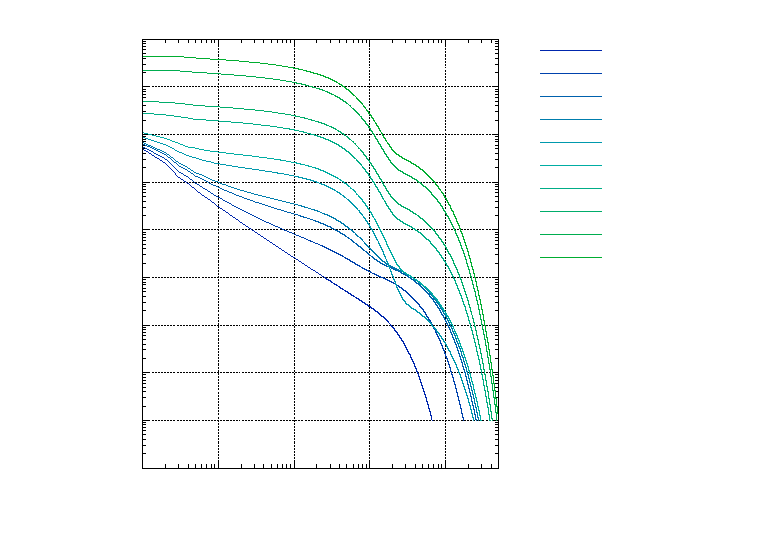
\includegraphics{GaussSeidel_delta}}%
    \gplfronttext
  \end{picture}%
\endgroup

		}
		\caption{The figure shows a plot of the infinity norm of the $ k $th residual, $ \|r^{(k)}\| $, against the number of iterations, $ k $. It can be seen that generally, as $ \delta $ gets larger, the number of iterations required to get the residual norm below the tolerance \texttt{TOL} increases logarithmically.\label{Fig:DeltaPlot}}
	\end{center}
\end{figure}
\newline\noindent
It can be seen in Figure \ref{Fig:DeltaPlot} that as $ \delta $ gets increasingly larger, the number of iterations required for the residual norm to get below the required tolerance, \texttt{TOL} = $ 10^{-6} $, gets expontentially larger. This can be explained since as we increase $ \delta $, the spectral raidus of the matrix $ B := P^{-1}N $ (chosen as in the introduction) gets increasingly larger, and since the asymptotic rate of convergence, $ R_{\infty} $, of the scheme is given by $ R_{\infty} := - \log\rho(B) $, where $ \rho(B) $ denotes the spectral radius of $ B $, the rate of convergence decreases and hence the number of iterations required to reach the tolerance increases.
\begin{figure}[h!]
	\begin{center}
		\textbf{Plot of residual norm against number of iterations for varying $ \lambda $}\par\medskip
		\resizebox{\linewidth}{\height}
		{
		% GNUPLOT: LaTeX picture with Postscript
\begingroup
  \makeatletter
  \providecommand\color[2][]{%
    \GenericError{(gnuplot) \space\space\space\@spaces}{%
      Package color not loaded in conjunction with
      terminal option `colourtext'%
    }{See the gnuplot documentation for explanation.%
    }{Either use 'blacktext' in gnuplot or load the package
      color.sty in LaTeX.}%
    \renewcommand\color[2][]{}%
  }%
  \providecommand\includegraphics[2][]{%
    \GenericError{(gnuplot) \space\space\space\@spaces}{%
      Package graphicx or graphics not loaded%
    }{See the gnuplot documentation for explanation.%
    }{The gnuplot epslatex terminal needs graphicx.sty or graphics.sty.}%
    \renewcommand\includegraphics[2][]{}%
  }%
  \providecommand\rotatebox[2]{#2}%
  \@ifundefined{ifGPcolor}{%
    \newif\ifGPcolor
    \GPcolorfalse
  }{}%
  \@ifundefined{ifGPblacktext}{%
    \newif\ifGPblacktext
    \GPblacktexttrue
  }{}%
  % define a \g@addto@macro without @ in the name:
  \let\gplgaddtomacro\g@addto@macro
  % define empty templates for all commands taking text:
  \gdef\gplbacktext{}%
  \gdef\gplfronttext{}%
  \makeatother
  \ifGPblacktext
    % no textcolor at all
    \def\colorrgb#1{}%
    \def\colorgray#1{}%
  \else
    % gray or color?
    \ifGPcolor
      \def\colorrgb#1{\color[rgb]{#1}}%
      \def\colorgray#1{\color[gray]{#1}}%
      \expandafter\def\csname LTw\endcsname{\color{white}}%
      \expandafter\def\csname LTb\endcsname{\color{black}}%
      \expandafter\def\csname LTa\endcsname{\color{black}}%
      \expandafter\def\csname LT0\endcsname{\color[rgb]{1,0,0}}%
      \expandafter\def\csname LT1\endcsname{\color[rgb]{0,1,0}}%
      \expandafter\def\csname LT2\endcsname{\color[rgb]{0,0,1}}%
      \expandafter\def\csname LT3\endcsname{\color[rgb]{1,0,1}}%
      \expandafter\def\csname LT4\endcsname{\color[rgb]{0,1,1}}%
      \expandafter\def\csname LT5\endcsname{\color[rgb]{1,1,0}}%
      \expandafter\def\csname LT6\endcsname{\color[rgb]{0,0,0}}%
      \expandafter\def\csname LT7\endcsname{\color[rgb]{1,0.3,0}}%
      \expandafter\def\csname LT8\endcsname{\color[rgb]{0.5,0.5,0.5}}%
    \else
      % gray
      \def\colorrgb#1{\color{black}}%
      \def\colorgray#1{\color[gray]{#1}}%
      \expandafter\def\csname LTw\endcsname{\color{white}}%
      \expandafter\def\csname LTb\endcsname{\color{black}}%
      \expandafter\def\csname LTa\endcsname{\color{black}}%
      \expandafter\def\csname LT0\endcsname{\color{black}}%
      \expandafter\def\csname LT1\endcsname{\color{black}}%
      \expandafter\def\csname LT2\endcsname{\color{black}}%
      \expandafter\def\csname LT3\endcsname{\color{black}}%
      \expandafter\def\csname LT4\endcsname{\color{black}}%
      \expandafter\def\csname LT5\endcsname{\color{black}}%
      \expandafter\def\csname LT6\endcsname{\color{black}}%
      \expandafter\def\csname LT7\endcsname{\color{black}}%
      \expandafter\def\csname LT8\endcsname{\color{black}}%
    \fi
  \fi
    \setlength{\unitlength}{0.0500bp}%
    \ifx\gptboxheight\undefined%
      \newlength{\gptboxheight}%
      \newlength{\gptboxwidth}%
      \newsavebox{\gptboxtext}%
    \fi%
    \setlength{\fboxrule}{0.5pt}%
    \setlength{\fboxsep}{1pt}%
\begin{picture}(7200.00,5040.00)%
    \gplgaddtomacro\gplbacktext{%
      \csname LTb\endcsname%%
      \put(1078,1078){\makebox(0,0)[r]{\strut{}1e-10}}%
      \csname LTb\endcsname%%
      \put(1078,1826){\makebox(0,0)[r]{\strut{}1e-08}}%
      \csname LTb\endcsname%%
      \put(1078,2574){\makebox(0,0)[r]{\strut{}1e-06}}%
      \csname LTb\endcsname%%
      \put(1078,3323){\makebox(0,0)[r]{\strut{}1e-04}}%
      \csname LTb\endcsname%%
      \put(1078,4071){\makebox(0,0)[r]{\strut{}1e-02}}%
      \csname LTb\endcsname%%
      \put(1078,4819){\makebox(0,0)[r]{\strut{}1e+00}}%
      \csname LTb\endcsname%%
      \put(1210,484){\makebox(0,0){\strut{}$1$}}%
      \csname LTb\endcsname%%
      \put(3988,484){\makebox(0,0){\strut{}$10$}}%
    }%
    \gplgaddtomacro\gplfronttext{%
      \csname LTb\endcsname%%
      \put(198,2761){\rotatebox{-270}{\makebox(0,0){\strut{}$\| r^{(k)} \|_{\infty}$}}}%
      \put(2919,154){\makebox(0,0){\strut{}$k$}}%
      \csname LTb\endcsname%%
      \put(5747,4709){\makebox(0,0)[l]{\strut{}$\lambda = 1$}}%
      \csname LTb\endcsname%%
      \put(5747,4489){\makebox(0,0)[l]{\strut{}$\lambda = 10$}}%
      \csname LTb\endcsname%%
      \put(5747,4269){\makebox(0,0)[l]{\strut{}$\lambda = 50$}}%
      \csname LTb\endcsname%%
      \put(5747,4049){\makebox(0,0)[l]{\strut{}$\lambda = 100$}}%
      \csname LTb\endcsname%%
      \put(5747,3829){\makebox(0,0)[l]{\strut{}$\lambda = 500$}}%
      \csname LTb\endcsname%%
      \put(5747,3609){\makebox(0,0)[l]{\strut{}$\lambda = 1000$}}%
      \csname LTb\endcsname%%
      \put(5747,3389){\makebox(0,0)[l]{\strut{}$\lambda = 5000$}}%
      \csname LTb\endcsname%%
      \put(5747,3169){\makebox(0,0)[l]{\strut{}$\lambda = 10000$}}%
      \csname LTb\endcsname%%
      \put(5747,2949){\makebox(0,0)[l]{\strut{}$\lambda = 50000$}}%
      \csname LTb\endcsname%%
      \put(5747,2729){\makebox(0,0)[l]{\strut{}$\lambda = 100000$}}%
    }%
    \gplbacktext
    \put(0,0){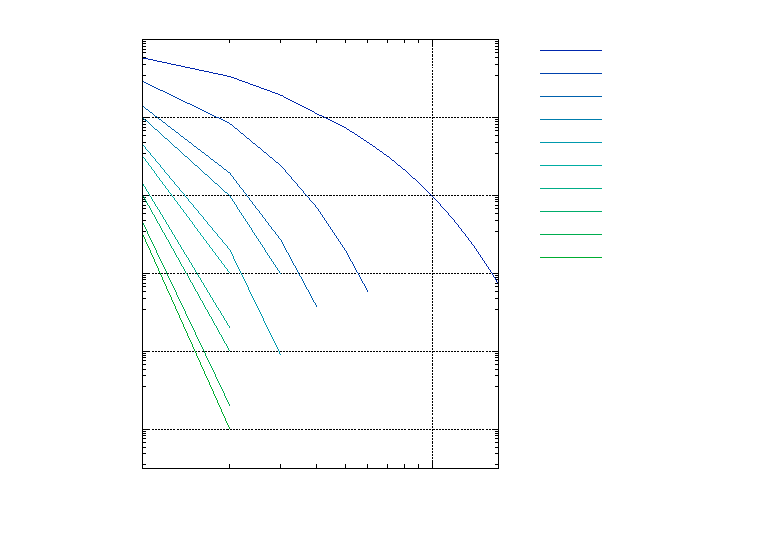
\includegraphics{GaussSeidel_lambda}}%
    \gplfronttext
  \end{picture}%
\endgroup

		}
		\caption{The figure shows a plot of the infinity norm of the $ k $th residual, $ \|r^{k}\| $, against the number of iterations, $ k $. We notice that as $ \lambda $ gets larger, the number of iterations required to get the residual norm below the tolerance \texttt{TOL} decreases. \label{Fig:LambdaPlot}}
	\end{center}
\end{figure}
\noindent
Furthermore, in Figure \ref{Fig:LambdaPlot}, we observe that as $ \lambda $ gets larger, the number of iterations required for the residual norm to be below the required tolerance rapidly decreases. A possible explanation of this is that as $ \lambda $ gets very large, the order of the matrix $ \lambda I $ exceeds that of $ A $, and hence the resulting matrix $ B = A + \lambda I $ looks more and more like $ \lambda I $, decreasing the spectral radius of $ P^{-1}N $, and hence by a similar argument to that of $ \delta $ will result in less iterations being required to reach the tolerance.

%\subsection{$ N = 1,000 $}
%We now show results for when the algorithm is run when the matrix $ A $, given at the beginning of this section, is of size $ N = 1000 $. The results are given in Table \ref{Table:N1000} for varying values of $ \delta $ and $ \lambda $.
%\begin{table}[h!]
%\begin{minipage}{0.45\linewidth}
%		\begin{center}
%			\begin{tabular}{c|c|c|c}
%				$ \delta $ & $ \lambda $ & $ k $ & Error  \\
%				\hline 
%				1 & 0 & 186647 & 0.101512 \\  
%				10 & 0 & 726309 &  \\ 
%				50 & 0 & 1449582 & \\
%				100 & 0 & 1819726 & \\
%				500 & 0 & 2541927 & \\
%				1000 & 0 & 2675626 & \\
%				5000 & 0 & 1863905 & \\
%				10000 & 0 & 3180647 & \\
%				50000 & 0 & 4388590 & \\
%				100000 & 0 & 4808728 & \\
%			\end{tabular}	
%		\end{center}
%\end{minipage}
%\begin{minipage}{0.45\linewidth}
%		\begin{center}
%			\begin{tabular}{c|c|c}
%				$ \delta $ & $ \lambda $ & $ k $ \\
%				\hline 
%				1 & 1 & 17 \\  
%				1 & 10 & 6 \\ 
%				1 & 50 & 4 \\
%				1 & 100 & 3 \\
%				1 & 500 & 3 \\
%				1 & 1000 & 2 \\
%				1 & 5000 & 2 \\
%				1 & 10000 & 2 \\
%				1 & 50000 & 2 \\
%				1 & 100000 & 2 \\
%			\end{tabular}	
%		\end{center}
%\end{minipage}
%\caption{Iteration and error results for when $ N = 1000 $ for varying values of $ \delta $ and $ \lambda $. \label{Table:N1000}}
%\end{table}
%
%
%\subsection{$ N = 10,000 $}
%As was done for the case when $ N = 1000 $, we also present results for when $ N = 10000 $ in Table \ref{Table:N10000} below.
%\begin{table}[h!]
%	\begin{minipage}{0.45\linewidth}
%		\begin{center}
%			\begin{tabular}{c|c|c|c}
%				$ \delta $ & $ \lambda $ & $ k $ & Error  \\
%				\hline 
%				1 & 0 & 242319 & 0.819303 \\  
%				10 & 0 & 886252 &  \\ 
%				50 & 0 & 1449582 & \\
%				100 & 0 & 1819726 & \\
%				500 & 0 & 2541927 & \\
%				1000 & 0 & 2675626 & \\
%				5000 & 0 & 1863905 & \\
%				10000 & 0 & 3180647 & \\
%				50000 & 0 & 4388590 & \\
%				100000 & 0 & 4808728 & \\
%			\end{tabular}	
%		\end{center}
%	\end{minipage}
%	\begin{minipage}{0.45\linewidth}
%		\begin{center}
%			\begin{tabular}{c|c|c}
%				$ \delta $ & $ \lambda $ & $ k $ \\
%				\hline 
%				1 & 1 & 17 \\  
%				1 & 10 & 6 \\ 
%				1 & 50 & 4 \\
%				1 & 100 & 3 \\
%				1 & 500 & 3 \\
%				1 & 1000 & 2 \\
%				1 & 5000 & 2 \\
%				1 & 10000 & 2 \\
%				1 & 50000 & 2 \\
%				1 & 100000 & 2 \\
%			\end{tabular}	
%		\end{center}
%	\end{minipage}
%\caption{Iteration and error results for when $ N = 10000 $ for varying values of $ \delta $ and $ \lambda $. \label{Table:N10000}}
%\end{table}

\section{Conclusion}
\begin{table}
	\begin{center}
		\begin{tabular}{c|c|c}
			Size of matrix $ N $ & Number of iterations $ k $ & Error \\
			\hline
			100 & 6664 & 0.00103237 \\
			1000 & 186647 & 0.101512 \\
			10000 & 242319 & 0.819303
		\end{tabular}
	\end{center}
	\caption{Comparing the number of iterations required to reach the required tolerance, $ 10^{-6} $, along with the error of the aquired solution to the real solution for three different values of $ N $.\label{Talbe:NComparison}}
\end{table}
The \texttt{GaussSeidel} numerical scheme works successfully and quite rapidly, even when $ N $ is very large, but one can see from Table \ref{Talbe:NComparison} that the error between the exact solution and the result of the iterative scheme in the maximum norm increases with $ N $. Therefore it would be wise, when dealing with extemely large matrices, one adopts an improved numerical scheme as to obtain more accurate solutions. One could obtain more accurate solutions with the above \texttt{GaussSeidel} implementation by chooing an even smaller tolerance for the residual norm, since the norm of the error is related to the residual norm, but this would be done with sacrifice to computation time, which is not a problem if one is patient enough. The implementation of Gauss-Seidel could also be altered to improve the speed of algorithm by removing the use of \texttt{getEntry} in the \texttt{GaussSeidel} function. This could possibly increase the speed of the execution since it would not require the algorithm to call \texttt{getEntry} at every look within an iteration. We could further increase the performance by storing the indices of entries in order when calling \texttt{addEntry}, and then implementing a smarter ``\texttt{getEntry}" type loop within \texttt{GaussSeidel}.

%\section*{Introduction}

\end{document}
